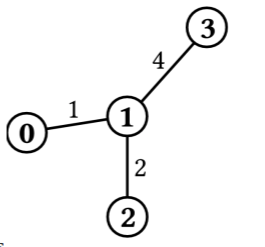
\includegraphics{race1.png}

Трасса может начинаться в городе с номером $0$, проходить через город c номером $1$ и закончиться в городе c номером $2$. Длина трассы будет равна $1 + 2 = 3$ км, как и требуется, и она состоит из двух магистралей. Это наилучшая возможная трасса; поэтому процедура \t{best\_path(N,K,H,L)} должна вернуть значение $2$.

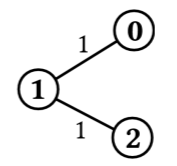
\includegraphics{race2.png}

Здесь допустимой трассы не существует. В этом примере процедура \t{best\_path(N,K,H,L)} должна вернуть значение $-1$.

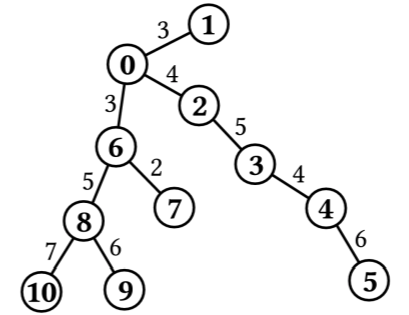
\includegraphics{race3.png}

Одна из возможных трасс состоит из $3$ магистралей: она идёт из города с номером $6$ через города с номерами $0$ и $2$ в город c номером $3$. Другая трасса начинается в городе с номером $10$ и идёт через город с номером $8$ в город с номером $6$. Обе эти трассы имеют длину $12$ километров, как и требуется. Вторая из них оптимальна, так как не существует подходящей трассы из одной магистрали. Таким образом, процедура \t{best\_path(N,K,H,L)} должна вернуть значение $2$.
